% ==========================================
% Section 9: Feature Subset Selection (Slides 39-48)
% ==========================================

% Slide 39: High Dimensionality
\begin{frame}{ابعاد بالا (\lr{High Dimensionality})}
\begin{columns}[c]
  \begin{column}{0.55\textwidth}
    \begin{itemize}
      \item \textbf{مجموعه داده‌هایی با تعداد بسیار زیادی ویژگی:}
      \begin{itemize}
        \item دسته‌بندی متون (هزاران کلمه)
        \item پردازش و بینایی تصویر (میلیون‌ها پیکسل)
        \item داده‌های بیان ژن و ژنومیک (ده‌ها هزار ژن با تعداد نمونه‌های کم)
      \end{itemize}
      \vspace{0.2cm}
      \item \textbf{پیامدهای ابعاد بالا:}
      \begin{itemize}
        \item افزایش تصاعدی هزینه محاسباتی
        \item خطر بسیار بالای بیش‌برازش (\lr{Overfitting})
        \item ناتوانی در تجسم و تفسیر روابط توسط انسان
      \end{itemize}
    \end{itemize}
  \end{column}
  \begin{column}{0.43\textwidth}
    \centering
    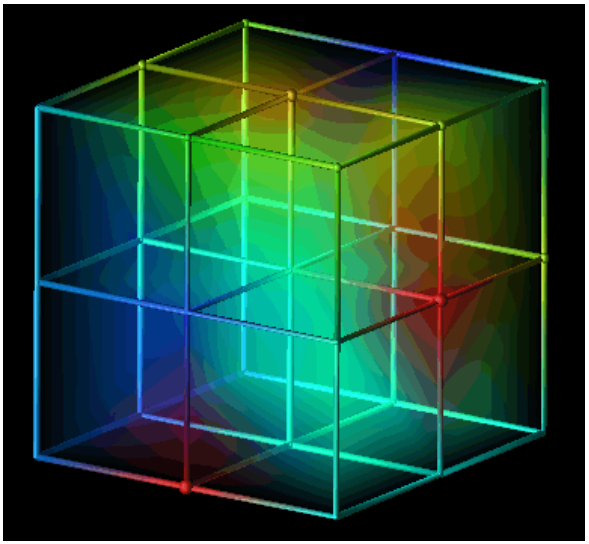
\includegraphics[width=\textwidth]{images/page_39_img_1.png}
  \end{column}
\end{columns}
\end{frame}

% Slide 40: Feature Subset Selection Goal
\begin{frame}{انتخاب زیرمجموعه ویژگی‌ها (\lr{Feature Subset Selection})}
\begin{itemize}
  \item \textbf{یک گام پیش‌پردازش حیاتی:}
  \begin{itemize}
    \item ایده اصلی: تنها ویژگی‌های ارزشمند و با بار اطلاعاتی بالا نگه‌داشته شوند.
    \item اصطلاح «ویژگی» (\lr{Feature}) در ادبیات یادگیری ماشین معادل همان «صفت/ویژگی» (\lr{Attribute}) است.
  \end{itemize}
  \vspace{0.3cm}
  \item \textbf{اهداف سه‌گانه انتخاب ویژگی:}
  \begin{itemize}
    \item بهبود دقت و قدرت تعمیم مدل (جلوگیری از یادگیری نویز)
    \item کاهش زمان آموزش و آزمایش الگوریتم‌ها
    \item تسهیل درک، تفسیر و توضیح‌پذیری مدل برای تصمیم‌گیرندگان انسانی
  \end{itemize}
\end{itemize}
\end{frame}

% Slide 41: Filter vs Wrapper Methods
\begin{frame}{دسته‌بندی اصلی: روش‌های فیلتری در برابر پوششی}
\begin{itemize}
  \item \textbf{تمایز بنیادین: روش‌های فیلتری در برابر روش‌های پوششی}
  \vspace{0.2cm}
  \item \textbf{روش‌های فیلتری (\lr{Filter Methods})}
  \begin{itemize}
    \item ارزیابی و رتبه‌بندی ویژگی‌ها بر مبنای معیارهای آماری مستقل از مدل یادگیری.
    \item استفاده از معیارهای وزن‌دهی نظیر آزمون کای-دو ($\chi^2$)، بهره اطلاعاتی (\lr{Information Gain})، و ضریب همبستگی.
    \item انتخاب ویژگی‌های دارای بالاترین امتیاز وزنی.
    \item سرعت محاسباتی بسیار بالا (خطی بر حسب تعداد ویژگی‌ها)، اما الزماً بهینه سراسری نیست.
  \end{itemize}
  \vspace{0.25cm}
  \item \textbf{نمونه کد پایتون (\lr{scikit-learn}):}
  \begin{itemize}
    \item انتخاب ۲۰ ویژگی برتر بر اساس آزمون آماری کای-دو:\\
    \vspace{0.1cm}
    \codebox{X\_f = SelectKBest(chi2, k=20).fit\_transform(X, y)}
  \end{itemize}
\end{itemize}
\end{frame}

% Slide 42: Filter Methods Details
\begin{frame}{روش‌های فیلتری: حذف ویژگی‌های زائد}
\begin{itemize}
  \item \textbf{حذف ویژگی‌های تکراری و زائد (\lr{Redundant Attributes})}
  \begin{itemize}
    \item به عنوان مثال: ثبت دما همزمان بر حسب سلسیوس و فارنهایت.
    \item ثبت ویژگی‌های متنی کاملاً هم‌رخداد (مانند نام «باراک» و «اوباما»).
  \end{itemize}
  \vspace{0.2cm}
  \item \textbf{معیارهای ارزیابی آماری در روش‌های فیلتری:}
  \begin{itemize}
    \item ضریب همبستگی پیرسون / اسپیرمن بین ویژگی و متغیر هدف
    \item معیار اطلاعات متقابل (\lr{Mutual Information})
    \item آزمون آماری کای-دو (\lr{Chi-Square Test}) برای ویژگی‌های گسسته
    \item آستانه حداقل واریانس (\lr{Variance Threshold})
  \end{itemize}
  \vspace{0.2cm}
  \item \textbf{مزیت بزرگ:} سرعت محاسباتی فوق‌العاده بالا و مقیاس‌پذیری عالی.
\end{itemize}
\end{frame}

% Slide 43: Wrapper Methods Details
\begin{frame}{روش‌های پوششی (\lr{Wrapper Methods})}
\begin{itemize}
  \item \textbf{اصول کارکرد روش‌های پوششی:}
  \begin{itemize}
    \item یک مدل طبقه‌بند داخلی به عنوان جعبه سیاه ارزیاب به کار گرفته می‌شود.
    \item مدل با زیرمجموعه‌های متفاوتی از ویژگی‌ها آموزش دیده و دقت آن ارزیابی می‌شود.
    \item زیرمجموعه‌ای که بالاترین امتیاز اعتبارسنجی را کسب کند انتخاب می‌گردد.
  \end{itemize}
  \vspace{0.3cm}
  \item \textbf{چالش بنیادین:}
  \begin{itemize}
    \item فضای جستجو نمایی است: برای $n$ ویژگی، $2^n$ زیرمجموعه محتمل وجود دارد!
    \item جستجوی جامع (\lr{Exhaustive Search}) برای بیش از ۲۰ ویژگی غیرممکن است.
  \end{itemize}
\end{itemize}
\end{frame}

% Slide 44: Forward Selection
\begin{frame}{انتخاب پیش‌رو (\lr{Forward Selection})}
\begin{itemize}
  \item \textbf{الگوریتم انتخاب پیش‌رو حریصانه (\lr{Greedy Forward Selection})}
  \begin{enumerate}
    \item با مجموعه ویژگی خالی آغاز کنید.
    \item حلقه تکرار:
    \begin{itemize}
      \item به ازای هر ویژگی باقیمانده، آن را به طور موقت اضافه کنید و مدل را بسنجید.
      \item ویژگی‌ای را که بیشترین بهبود در کارایی مدل را ایجاد کند به صورت دائمی اضافه کنید.
    \end{itemize}
    \item شرط توقف: زمانی که افزودن هیچ ویژگی جدیدی موجب بهبود معنادار مدل نشود.
  \end{enumerate}
  \vspace{0.3cm}
  \item \textbf{پیچیدگی محاسباتی:} از مرتبه $O(n^2)$ به جای $O(2^n)$، بسیار سریع‌تر اما ممکن است به بهینه محلی همگرا شود.
\end{itemize}
\end{frame}

% Slide 45: Backward Elimination
\begin{frame}{حذف پس‌رو (\lr{Backward Elimination})}
\begin{itemize}
  \item \textbf{الگوریتم حذف پس‌رو (\lr{Greedy Backward Elimination})}
  \begin{enumerate}
    \item با مجموعه تمام ویژگی‌ها آغاز کنید.
    \item حلقه تکرار:
    \begin{itemize}
      \item به ازای هر ویژگی موجود در مجموعه، آن را موقتاً حذف کرده و مدل را بسنجید.
      \item ویژگی‌ای را که حذف آن کمترین افت کارایی (یا حتی بهبود مدل) را به همراه دارد حذف کنید.
    \end{itemize}
    \item شرط توقف: زمانی که حذف هر یک از ویژگی‌های باقیمانده باعث افت فاحش در کارایی مدل گردد.
  \end{enumerate}
  \vspace{0.3cm}
  \item \textbf{نکته:} قادر به در نظر گرفتن برهم‌کنش‌های اولیه بین تمام متغیرها است، اما در شروع برای ابعاد بزرگ بسیار کند است.
\end{itemize}
\end{frame}

% Slide 46: Checkerboard Dataset
\begin{frame}{مجموعه داده صفحه شطرنجی (\lr{Checkerboard Dataset})}
\begin{columns}[c]
  \begin{column}{0.55\textwidth}
    \begin{itemize}
      \item \textbf{چالش تعاملات غیرخطی:}
      \begin{itemize}
        \item درخت تصمیم و روش‌های پوششی به راحتی مرزهای این مسئله شطرنجی را یاد می‌گیرند.
        \item اما اگر از روش فیلتری تک‌متغیره استفاده کنیم چه می‌شود؟
        \item هیچ‌یک از دو بعد $X$ یا $Y$ به تنهایی همبستگی خطی با کلاس هدف ندارند!
        \item روش‌های فیلتری ممکن است هر دو ویژگی ضروری را نادیده بگیرند!
      \end{itemize}
    \end{itemize}
  \end{column}
  \begin{column}{0.43\textwidth}
    \centering
    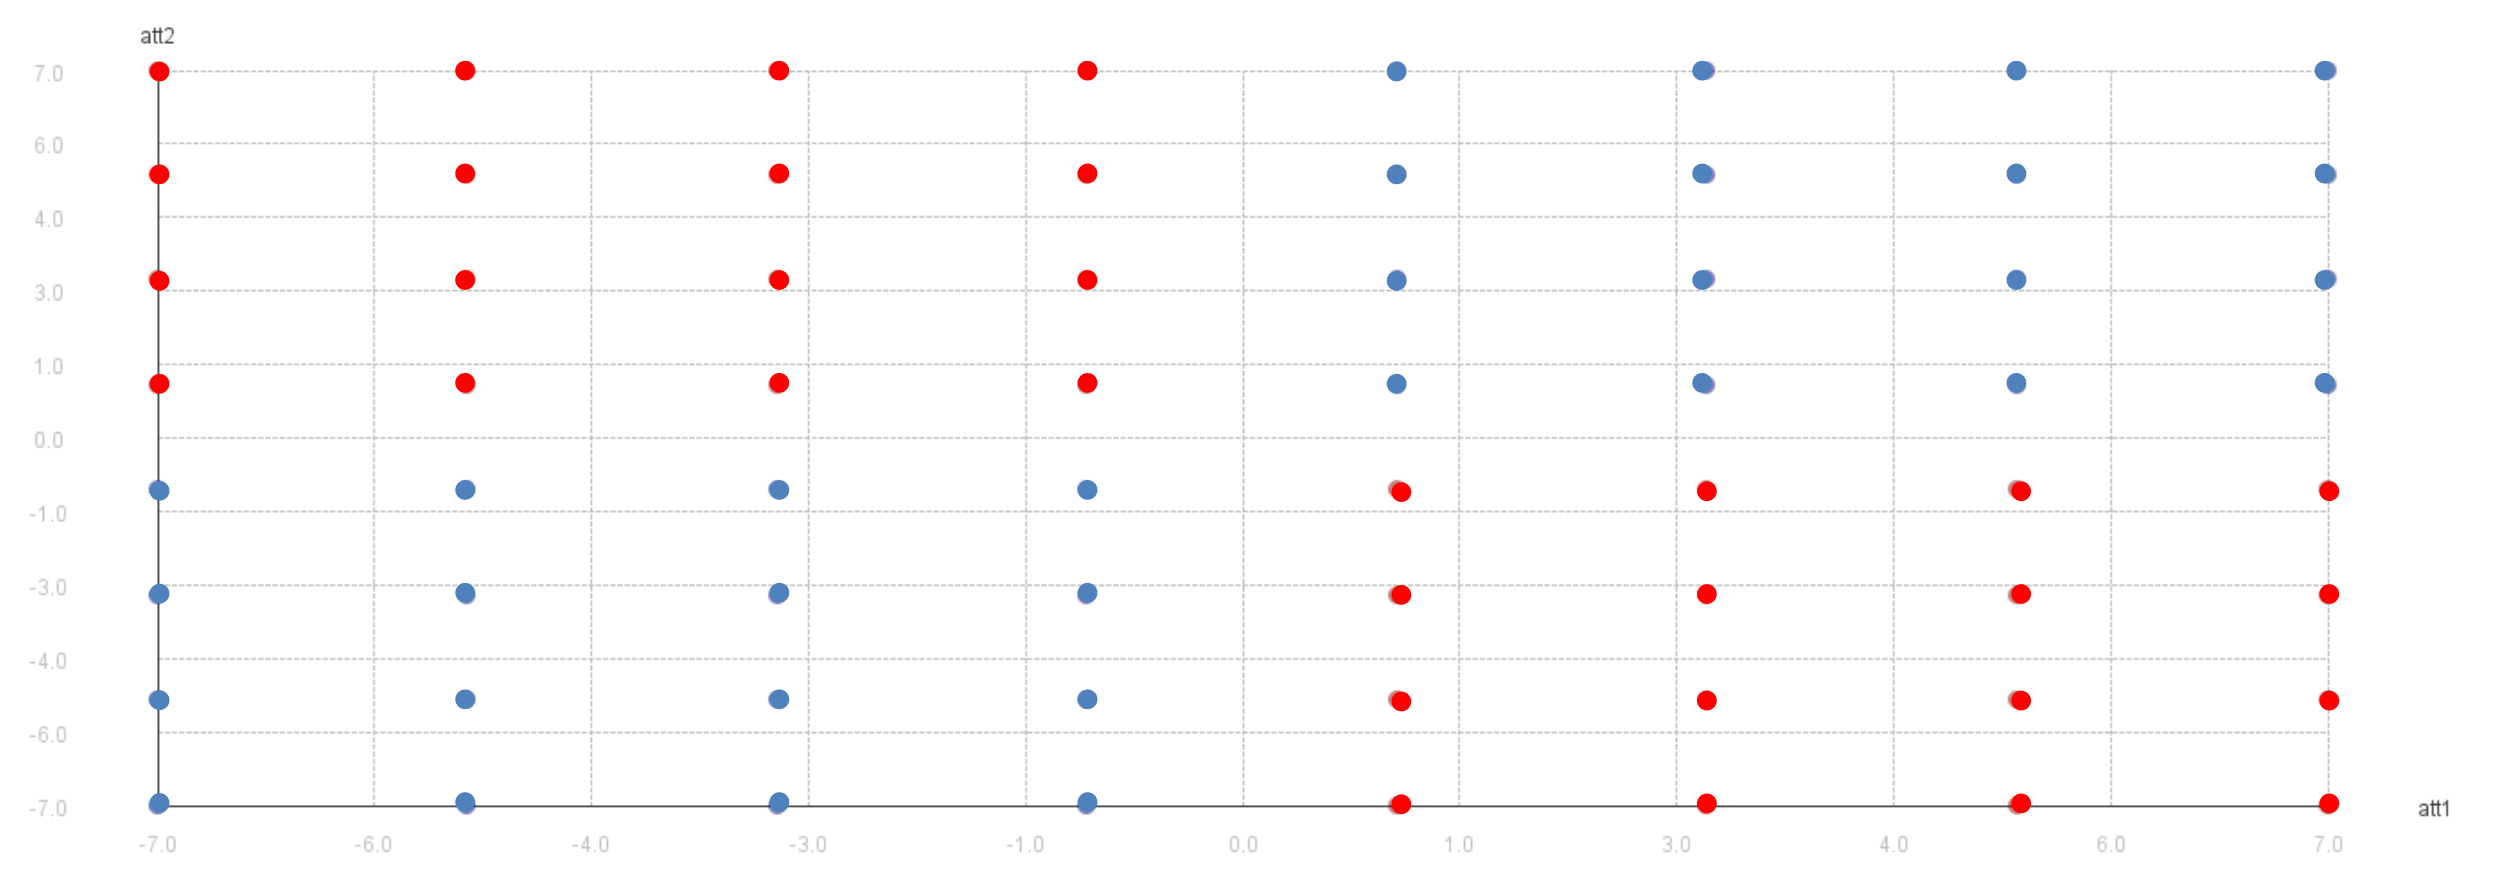
\includegraphics[width=\textwidth]{images/page_46_img_1.png}
  \end{column}
\end{columns}
\end{frame}

% Slide 47: Python Implementation
\begin{frame}{پیاده‌سازی انتخاب ویژگی در پایتون (\lr{scikit-learn})}
\begin{itemize}
  \item \textbf{روش‌های پوششی ترتیبی با \codeinline{SequentialFeatureSelector}:}
  \begin{itemize}
    \item \textbf{انتخاب پیش‌رو (\lr{Forward Selection}):}\\
    \vspace{0.06cm}
    \codebox{SequentialFeatureSelector(direction='forward')}
    \vspace{0.12cm}
    \item \textbf{حذف پس‌رو (\lr{Backward Elimination}):}\\
    \vspace{0.06cm}
    \codebox{SequentialFeatureSelector(direction='backward')}
  \end{itemize}
  \vspace{0.25cm}
  \item \textbf{در صورت دسترسی به اهمیت ویژگی‌ها در مدل (\lr{feature\_importances\_}):}
  \begin{itemize}
    \item حذف بازگشتی ویژگی با اعتبارسنجی متقاطع:\\
    \vspace{0.06cm}
    \codebox{RFECV(Recursive feature elimination with CV)}
    \vspace{0.12cm}
    \item اجرای یک گام غربالگری بر مبنای اهمیت صفات:\\
    \vspace{0.06cm}
    \codebox{SelectFromModel(estimator)}
  \end{itemize}
\end{itemize}
\end{frame}

% Slide 48: Further Approaches
\begin{frame}{سایر رویکردهای انتخاب ویژگی}
\begin{itemize}
  \item \textbf{جستجوی جامع (\lr{Brute Force Search})}
  \begin{itemize}
    \item تضمین یافتن بهترین زیرمجموعه ممکن، اما تنها تا حدود ۱۵ تا ۲۰ ویژگی قابل اجرا است.
  \end{itemize}
  \vspace{0.2cm}
  \item \textbf{الگوریتم‌های تکاملی و ژنتیک (\lr{Genetic / Evolutionary Algorithms})}
  \begin{itemize}
    \item جستجوی هوشمندانه در فضای ترکیبیاتی با عملگرهای جهش و تقاطع کروموزوم‌ها.
  \end{itemize}
  \vspace{0.2cm}
  \item \textbf{روش‌های توکار (\lr{Embedded Methods})}
  \begin{itemize}
    \item انتخاب ویژگی به عنوان بخشی ذاتی از فرآیند یادگیری مدل (مانند جریمه‌سازی \lr{Lasso / L1} و اهمیت ویژگی‌ها در درخت‌های تصمیم و \lr{Random Forest}).
  \end{itemize}
\end{itemize}
\end{frame}
